\section{Exercises on Matching Problems}

\subsection{Problem 4.1. Scheduling Technicians}

\paragraph{}
\begin{quote}
GTC employs fifteen maintenance technicians who are used to solve problems that
customers have with their communication devices. The technicians are paid by hours
of work. All technicians have the same wage per hour, but are not equally qualified
on all problems. The problems are divided into ten different categories. This morning,
twenty customers have problems in the categories shown in Table \ref{cuscat}. However
only fifteen customers can be served, because each technician is assigned to only
one job. The twenty customers have called in the order 1 through 20, meaning that
Customer 1 has called first, and Customer 20 called last. The time required by a technician to solve a problem is called the repairing time. Assume that GTC knows the
repairing times per category and per technician. These times are shown in Table \ref{techcattimes}.
For example, Technician 2 needs 17 minutes to solve a problem in Category 1. GTC
wants to serve fifteen customers at minimum technician wage cost.\end{quote}

\begin{table}[H]
	\centering
	\caption{Customers and their categories}
	\begin{tabular}{cc||cc||cc}\hline
	Customer & Category & Customer & Category & Customer & Category \\ \hline
	1&1&8&2&15&7\\
	2&6&9&7&16&9\\
	3&3&10&4&17&4\\
	4&7&11&5&18&7\\
	5&5&12&3&19&2\\
	6&8&13&9&20&1\\
	7&9&14&10&&\\ \hline
	\end{tabular}
	\label{cuscat}
\end{table}

\begin{table}[H]
	\centering
	\caption{Repairing times per technician per category}
	\begin{tabular}{c|*{10}c}\hline
	\multirow{2}{*}{Technicians} & \multicolumn{10}{|c}{Category} \\ \cline{2-11}
	& 1&2&3&4&5&6&7&8&9&10\\ \hline
	1&26&76&159&187&41&45&193&49&174&201\\
	2&17&91&128&162&50&42&167&38&146&122\\
	3&28&111&152&145&51&52&212&44&156&221\\
	4&24&84&155&209&58&44&146&41&122&177\\
	5&26&85&139&201&66&51&144&44&164&190\\
	6&21&95&176&197&65&58&196&52&157&209\\
	7&19&96&173&183&54&50&192&50&97&192\\
	8&19&84&135&177&52&45&175&42&99&212\\
	9&17&98&119&178&58&46&194&38&178&158\\
	10&24&80&109&199&60&50&218&61&142&150\\
	11&18&88&146&178&57&48&159&48&156&190\\
	12&28&105&124&158&55&43&150&36&132&183\\
	13&22&102&129&157&48&57&233&50&158&155\\
	14&28&110&168&217&48&58&159&47&136&179\\
	15&24&98&123&181&54&49&112&44&196&135\\ \hline
	\end{tabular}
	\label{techcattimes}
\end{table}

\begin{enumerate}[(a)]
\item\begin{quote}Assume that the customers are served on a first-call-first-served basis.\end{quote}
\begin{enumerate}[1.]
\item\begin{quote}By inspection, how would you assign the fifteen technicians to the customers?
What is the rationale behind your solution procedure?\end{quote}

	\paragraph{}
	The immediate solution would be to assign to the current customer the best available technician in customer's problem category. This greedy approach gives optimal solution when there is only one customer and tends to minimize expenses using the best available option at each step. The main advantage of the greedy solution is that it's really fast and easy to implement since all we need to do is to find minimum repairing time among 15 technicians 15 times. The assignment is shown in Table \ref{greedy-1-a}. The total repairing time equals 1,535.

\begin{table}[H]
	\centering
	\caption{Greedy assignment for first-call-first-served scheme}
	\begin{tabular}{|c|c|c|}\hline
	Customer & Technician & Repairing time \\ \hline
1 & 2 & 17 \\
2 & 12 & 43 \\
3 & 10 & 109 \\
4 & 15 & 112 \\
5 & 1 & 41 \\
6 & 9 & 38 \\
7 & 7 & 97 \\
8 & 4 & 84 \\
9 & 5 & 144 \\
10 & 3 & 145 \\
11 & 13 & 48 \\
12 & 8 & 135 \\
13 & 14 & 136 \\
14 & 11 & 190 \\
15 & 6 & 196 \\
\hline
	\end{tabular}
	\label{greedy-1-a}
\end{table}

\item\begin{quote}Explain why your solution need not be optimal.\end{quote}

	\paragraph{}
	The greedy approach doesn't necessary lead to an optimal solution. On the contrary, sometimes it can lead to the solution that is very far from being optimal. But nevertheless the greedy approach is a popular choice when the expenses of finding an optimal solution are higher than possible excess cost of a greedy strategy.

\item\begin{quote}What is an optimal assignment of technicians to customers, and what is the
total repairing time?\end{quote}

	\paragraph{}
	In order to find an optimal solution we should solve the so-called ``Assignment Problem'' (AP) \ref{burkard12}.

	\paragraph{}
	Let's consider a graph with vertices corresponding to technicians and customers. Between each pair of vertices where one corresponds to the technician A and other --- to the customer B there is an edge with an assigned weight that is equal to repairing time needed to technician A to handle the problem of the customer B (considering category of the problem of this customer). This graph is bipartite with technicians in the first part and customers in the second since there are edges only from technicians to customers. Moreover, we have a complete bipartite graph because there is an edge between every technician vertex and every customer vertex.

	\paragraph{}
	To solve an Assignment Problem means to find a perfect matching with minimum cost in this graph. Indeed, in a perfect matching every technician is assigned to a single customer and visa versa every customer has a single technician working on his problem and among all such matchings we choose the one with the minimum sum of edges --- minimum total repairing time because our expenses are proportional to it.

	\paragraph{}
	The AP can be efficiently solved by the Hungarian algorithm \ref{burkard12}. The input graph for Hungarian algorithm is given as an $15\times 15$ table where rows correspond to technicians and columns correspond to customers. The value in $i$-th row and $j$-th column represents the repairing time needed for technician $i$ to handle the problem of the customer $j$ (considering its category). The graph is shown in the Table \ref{graph-1-a}.

\begin{table}[H]
	\centering
	\caption{Input matrix for a Hungarian algorithm}
	\begin{tabular}{|*{16}{c|}}\hline
\backslashbox{Tech.}{Cust.} & 1 & 2 & 3 & 4 & 5 & 6 & 7 & 8 & 9 & 10 & 11 & 12 & 13 & 14 & 15\\\hline
1 & 26  & 45  & 159  & 193  & 41  & 49  & 174  & 76  & 193  & 187  & 41  & 159  & 174  & 201  & 193 \\ \hline
2 & 17  & 42  & 128  & 167  & 50  & 38  & 146  & 91  & 167  & 162  & 50  & 128  & 146  & 122  & 167 \\ \hline
3 & 28  & 52  & 152  & 212  & 51  & 44  & 156  & 111  & 212  & 145  & 51  & 152  & 156  & 221  & 212 \\ \hline
4 & 24  & 44  & 155  & 146  & 58  & 41  & 122  & 84  & 146  & 209  & 58  & 155  & 122  & 177  & 146 \\ \hline
5 & 26  & 51  & 139  & 144  & 66  & 44  & 164  & 85  & 144  & 201  & 66  & 139  & 164  & 190  & 144 \\ \hline
6 & 21  & 58  & 176  & 196  & 65  & 52  & 157  & 95  & 196  & 197  & 65  & 176  & 157  & 209  & 196 \\ \hline
7 & 19  & 50  & 173  & 192  & 54  & 50  & 97  & 96  & 192  & 183  & 54  & 173  & 97  & 192  & 192 \\ \hline
8 & 19  & 45  & 135  & 175  & 52  & 42  & 99  & 84  & 175  & 177  & 52  & 135  & 99  & 212  & 175 \\ \hline
9 & 17  & 46  & 119  & 194  & 58  & 38  & 178  & 98  & 194  & 178  & 58  & 119  & 178  & 158  & 194 \\ \hline
10 & 24  & 50  & 109  & 218  & 60  & 61  & 142  & 80  & 218  & 199  & 60  & 109  & 142  & 150  & 218 \\ \hline
11 & 18  & 48  & 146  & 159  & 57  & 48  & 156  & 88  & 159  & 178  & 57  & 146  & 156  & 190  & 159 \\ \hline
12 & 28  & 43  & 124  & 150  & 55  & 36  & 132  & 105  & 150  & 158  & 55  & 124  & 132  & 183  & 150 \\ \hline
13 & 22  & 57  & 129  & 233  & 48  & 50  & 158  & 102  & 233  & 157  & 48  & 129  & 158  & 155  & 233 \\ \hline
14 & 28  & 58  & 168  & 159  & 48  & 47  & 136  & 110  & 159  & 217  & 48  & 168  & 136  & 179  & 159 \\ \hline
15 & 24  & 49  & 123  & 112  & 54  & 44  & 196  & 98  & 112  & 181  & 54  & 123  & 196  & 135  & 112 \\
\hline
	\end{tabular}
	\label{graph-1-a}
\end{table}

	\paragraph{}
	The optimal assignment is shown in the Table \ref{hungarian-1-a}. The total repairing time equals 1,370 which is clearly lower than the one obtained using greedy strategy.

\begin{table}[H]
	\centering
	\caption{Optimal assignment for first-call-first-served scheme}
	\begin{tabular}{|c|c|c|}\hline
Customer & Technician & Repairing time \\ \hline
1 & 6 & 21 \\
2 & 11 & 48 \\
3 & 9 & 119 \\
4 & 5 & 144 \\
5 & 14 & 48 \\
6 & 12 & 36 \\
7 & 7 & 97 \\
8 & 1 & 76 \\
9 & 4 & 146 \\
10 & 3 & 145 \\
11 & 13 & 48 \\
12 & 10 & 109 \\
13 & 8 & 99 \\
14 & 2 & 122 \\
15 & 15 & 112 \\
\hline
	\end{tabular}
	\label{hungarian-1-a}
\end{table}

\end{enumerate}

\item\begin{quote}GTC now wants to analyze the consequences of serving fifteen customers out of
twenty for which the total wage is as low as possible.\end{quote}

\begin{enumerate}[1.]
\item\begin{quote}By inspection, how would you assign the fifteen technicians to the customers?
What is the rationale behind your solution procedure?\end{quote}

	\paragraph{}
	Once again the immediate thought would be to assign technicians greedily. But this time we are free to choose whom to serve first so instead of choosing the best technician for the next customer we will repeat the following procedure number of technicians times. On each iteration we will choose the best (in the sense of minimal repairing time) pair of technician and customer among currently unassigned technicians and customers. As the number of customers is greater than the number of technician and there is no fixed order of service neither for customers nor for technicians we can hope that the solution will be better than in the previous case since there are more possibilities for a good match. The assignment is shown in Table \ref{greedy-1-b}. The total repairing time equals 1,299. As we can see from Table \ref{greedy-1-b} customers 9, 14 and 15 who were served in part (a) are now left aside as there are more profitable matches for technicians. As we expected the resulting total repairing time is lower than in the previous case.

\begin{table}[H]
	\centering
	\caption{Greedy assignment when choosing among all the 20 customers}
	\begin{tabular}{|c|c|c|}\hline
Technician & Customer & Repairing time \\ \hline
1 & 5 & 41 \\
2 & 1 & 17 \\
3 & 10 & 145 \\
4 & 2 & 44 \\
5 & 3 & 139 \\
6 & 16 & 157 \\
7 & 7 & 97 \\
8 & 19 & 84 \\
9 & 20 & 17 \\
10 & 8 & 80 \\
11 & 12 & 146 \\
12 & 6 & 36 \\
13 & 11 & 48 \\
14 & 13 & 136 \\
15 & 4 & 112 \\
\hline
	\end{tabular}
	\label{greedy-1-b}
\end{table}


\item\begin{quote}Explain why your solution need not be optimal.\end{quote}

	\paragraph{}
	Even when there are more degrees of freedom for choosing the best variant of each iteration of the greedy algorithm it doesn't necessary lead to an optimal solution. Indeed, the greedy approach tries to optimize the problem locally --- considering only the current iteration and neither using information from the previous steps nor changing the already assigned pairs. But once again --- the greedy approach is very attractive because of it's simplicity.	

\item\begin{quote}Set up an optimization model to solve this problem.\end{quote}

	\paragraph{}
	Let's consider a complete bipartite graph $G=(T,C,E)$ with to set of vertices $T$ corresponding to technicians ($|T|=15$) and set of vertices $C$ corresponding to customers ($|C|=20$). Between each pair of vertices where one corresponds to the $i$-th technician and other --- to the $j$-th customer there is an edge with an assigned weight $w_{ij}$ that is equal to repairing time needed to technician $i$ to handle the problem of the customer $j$ (considering category of the problem of this customer). The cost matrix of this graph $W=\{w_{ij}\}$ is shown in Table \ref{graph-1-b}. As in \ref{graph-1-a} the rows correspond to technicians and columns correspond to customers.

\begin{table}[H]
	\centering
	\caption{Cost matrix $W$ for an optimal assignment problem of 15 technicians to 20 customers}
	\begin{tabular}{|*{21}{c|}}\hline
 $T$\textbackslash $C$ & 1 & 2 & 3 & 4 & 5 & 6 & 7 & 8 & 9 & 10 & 11 & 12 & 13 & 14 & 15 & 16 & 17 & 18 & 19 & 20\\\hline
1 & 26  & 45  & 159  & 193  & 41  & 49  & 174  & 76  & 193  & 187  & 41  & 159  & 174  & 201  & 193  & 174  & 187  & 193  & 76  & 26 \\ \hline
2 & 17  & 42  & 128  & 167  & 50  & 38  & 146  & 91  & 167  & 162  & 50  & 128  & 146  & 122  & 167  & 146  & 162  & 167  & 91  & 17 \\ \hline
3 & 28  & 52  & 152  & 212  & 51  & 44  & 156  & 111  & 212  & 145  & 51  & 152  & 156  & 221  & 212  & 156  & 145  & 212  & 111  & 28 \\ \hline
4 & 24  & 44  & 155  & 146  & 58  & 41  & 122  & 84  & 146  & 209  & 58  & 155  & 122  & 177  & 146  & 122  & 209  & 146  & 84  & 24 \\ \hline
5 & 26  & 51  & 139  & 144  & 66  & 44  & 164  & 85  & 144  & 201  & 66  & 139  & 164  & 190  & 144  & 164  & 201  & 144  & 85  & 26 \\ \hline
6 & 21  & 58  & 176  & 196  & 65  & 52  & 157  & 95  & 196  & 197  & 65  & 176  & 157  & 209  & 196  & 157  & 197  & 196  & 95  & 21 \\ \hline
7 & 19  & 50  & 173  & 192  & 54  & 50  & 97  & 96  & 192  & 183  & 54  & 173  & 97  & 192  & 192  & 97  & 183  & 192  & 96  & 19 \\ \hline
8 & 19  & 45  & 135  & 175  & 52  & 42  & 99  & 84  & 175  & 177  & 52  & 135  & 99  & 212  & 175  & 99  & 177  & 175  & 84  & 19 \\ \hline
9 & 17  & 46  & 119  & 194  & 58  & 38  & 178  & 98  & 194  & 178  & 58  & 119  & 178  & 158  & 194  & 178  & 178  & 194  & 98  & 17 \\ \hline
10 & 24  & 50  & 109  & 218  & 60  & 61  & 142  & 80  & 218  & 199  & 60  & 109  & 142  & 150  & 218  & 142  & 199  & 218  & 80  & 24 \\ \hline
11 & 18  & 48  & 146  & 159  & 57  & 48  & 156  & 88  & 159  & 178  & 57  & 146  & 156  & 190  & 159  & 156  & 178  & 159  & 88  & 18 \\ \hline
12 & 28  & 43  & 124  & 150  & 55  & 36  & 132  & 105  & 150  & 158  & 55  & 124  & 132  & 183  & 150  & 132  & 158  & 150  & 105  & 28 \\ \hline
13 & 22  & 57  & 129  & 233  & 48  & 50  & 158  & 102  & 233  & 157  & 48  & 129  & 158  & 155  & 233  & 158  & 157  & 233  & 102  & 22 \\ \hline
14 & 28  & 58  & 168  & 159  & 48  & 47  & 136  & 110  & 159  & 217  & 48  & 168  & 136  & 179  & 159  & 136  & 217  & 159  & 110  & 28 \\ \hline
15 & 24  & 49  & 123  & 112  & 54  & 44  & 196  & 98  & 112  & 181  & 54  & 123  & 196  & 135  & 112  & 196  & 181  & 112  & 98  & 24 \\ \hline
	\end{tabular}
	\label{graph-1-b}
\end{table}
	
	\paragraph{}
	Now the optimization problem for an optimal assignment can be stated as follows.
$$
	\textbf{Minimize}
$$
$$
	z = \sum\limits_{i\in T, j\in C} w_{ij}x_{ij}
$$
$$
	\textbf{Subject to}
$$
$$
	\sum\limits_{j\in C} x_{ij} \leq 1 \ \text{for each }i\in T
$$
$$
	x_{ij} \geq 0 \ \text{for each }i\in T,\  j\in C
$$

\item\begin{quote}What is an optimal assignment of technicians to customers now, and what is
the total repairing time?\end{quote}

	\paragraph{}
	The stated optimization problem is once again equivalent to the ``Assignment Problem'' and can be effectively solved using Hungarian algorithm using matrix $W$ as an input cost matrix. The optimal assignment is shown in the Table \ref{hungarian-1-b}. The total repairing time equals 1,163 which is lower than the one obtained using greedy strategy.

\begin{table}[H]
	\centering
	\caption{Optimal assignment problem of 15 technicians to 20 customers}
	\begin{tabular}{|c|c|c|}\hline
Technician & Customer & Repairing time \\ \hline
1 & 19 & 76 \\
2 & 14 & 122 \\
3 & 6 & 44 \\
4 & 16 & 122 \\
5 & 8 & 85 \\
6 & 1 & 21 \\
7 & 7 & 97 \\
8 & 13 & 99 \\
9 & 12 & 119 \\
10 & 3 & 109 \\
11 & 20 & 18 \\
12 & 2 & 43 \\
13 & 5 & 48 \\
14 & 11 & 48 \\
15 & 4 & 112 \\
\hline
	\end{tabular}
	\label{hungarian-1-b}
\end{table}

\end{enumerate}

\item\begin{quote}Why is the optimal solution to part (b) not worse than the optimal solution to part
(a) in terms of repair times?\end{quote}

	\paragraph{}
	The explanation is quite similar to that when we explained our expectations that the new greedy algorithm will yield better results. What have changed in part (b) comparing to part (a) is that we added 5 extra columns to the cost matrix. So in the worst case (when the values in the added columns are very high) we could just ignore them and stick to our previous solution of problem with $15\times15$ matrix. But in our case the values in these columns added extra degrees of freedom to our problem (more variant for each technician to choose from) so the Hungarian algorithm was able to make use of this extra values and improve the solution.

\item\begin{quote}Draw and analyze the perturbation function corresponding to the model used in
part (b), of the coefficient representing the time that Technician 2 needs to serve
Customer 14.\end{quote}

	\paragraph{}
	To draw the perturbation function we'll iterate through possible values of the repairing time needed for technician 2 to serve customer 14, or using the definitions above we'll iterate through values of $w_{2,14}$ and calculate the total repairing time of an optimal assignment using Hungarian algorithm. The perturbation function for $w_{2,14}=0,1,\dots,200$ is shown in the Figure \ref{perturbation2-14}.

\begin{figure}[H]
	\centering
	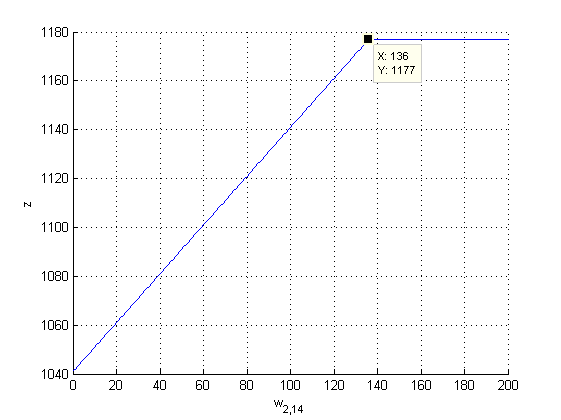
\includegraphics[scale=1]{./img/perturbation2-14.png}
	\caption{Perturbation function of the Assignment Problem for the parameter $w_{2,14}$}
	\label{perturbation2-14}
\end{figure}

	\paragraph{}
	From the Figure \ref{perturbation2-14} we can see that starting from $w_{2,14}=0$ technician 2 is assigned to customer 14 in an optimal solution. But starting from the value $w_{2,14}=136$ it's no longer mandatory to assign technician 2 to customer 14 in order to get an optimal value of objective function as an alternative equivalent solution arises. It's clear that further increase of $w_{2,14}$ won't return edge (2,~14) to the solution. Knowing perturbation function we are able to calculate the upper tolerance of parameter $w_{2,14}$ --- the maximal increase that leaves edge (2,~14) in the optimal solution. Upper tolerance of $w_{2,14}$ equals $1177 - 1163 = 136 - 122 = 14$.

\item\begin{quote}Based on the first-call-first-serve principle, what happens to the optimal solution
to part (a) when Technician 2 is not available and Technician 8 visits two
customers?\end{quote}

	\paragraph{}
	``Technician 2 is not available and technician 8 visits two customers'' is equivalent to ``technician 2 is replaced by technician 8''. Indeed, we still need to find optimal assignment with all 15 technicians occupied but instead of technician 2 we have technician 8 now. So we modify the cost matrix \ref{graph-1-a} in the corresponding manner by copying the row \#8 to the row \#2 and apply Hungarian algorithm to the new matrix. The optimal assignment is shown in the Table \ref{hungarian-1-e}. The total repairing time equals 1,404 which is greater than it was with technician 2 available. It's worth noting that even if all that we've done was replacing one row of matrix by the copy of another, the optimal solution required more serious changes than just replacing 2 with 8 in the assignment. Customer 5 is now served by technician 1 instead of 14, customer 8 switched from technician 1 to 8, customer 11 --- from 13 to 14 and customer 14 --- from 2 to 13.

\begin{table}[H]
	\centering
	\caption{Optimal assignment for first-call-first-served scheme with technician 2 replaced by technician 8}
	\begin{tabular}{|c|c|c|}\hline
Customer & Technician & Repairing time \\ \hline
1 & 6 & 21 \\
2 & 11 & 48 \\
3 & 9 & 119 \\
4 & 5 & 144 \\
5 & 1 & 41 \\
6 & 12 & 36 \\
7 & 7 & 97 \\
8 & 8 & 84 \\
9 & 4 & 146 \\
10 & 3 & 145 \\
11 & 14 & 48 \\
12 & 10 & 109 \\
13 & 8 & 99 \\
14 & 13 & 155 \\
15 & 15 & 112 \\
\hline
	\end{tabular}
	\label{hungarian-1-e}
\end{table}

\item\begin{quote}What happens to the optimal assignment of part (b) if Customer 4 solves the
problem himself, so that no technician is needed for this customer?\end{quote}

	\paragraph{}
	If the customer 4 no longer needs help than we just remove him from consideration when planning an assignment. In mathematical formulation --- we just delete the corresponding (4-th) column from the cost matrix \ref{graph-1-b}. After that we apply Hungarian algorithm to obtain an optimal solution. The optimal assignment is shown in the Table \ref{hungarian-1-f}. The total repairing time equals 1,163 which is equal to the total time of the optimal assignment from part (b). It's can be easily explained as the changes in the optimal assignment are minimal --- technician 15 who served customer 4 now serves customer 9, but customers 4 and 9 have exactly the same problem category so nothing changes from technician 15 and repairing time remains the same. And since customer 9 wasn't served in the optimal solution of part (b) the switch for technician 15 is painless.

\begin{table}[H]
	\centering
	\caption{Optimal assignment problem of 15 technicians to 19 customers (excluding customer 4)}
	\begin{tabular}{|c|c|c|}\hline
Technician & Customer & Repairing time \\ \hline
1 & 19 & 76 \\
2 & 14 & 122 \\
3 & 6 & 44 \\
4 & 16 & 122 \\
5 & 8 & 85 \\
6 & 1 & 21 \\
7 & 7 & 97 \\
8 & 13 & 99 \\
9 & 12 & 119 \\
10 & 3 & 109 \\
11 & 20 & 18 \\
12 & 2 & 43 \\
13 & 5 & 48 \\
14 & 11 & 48 \\
15 & 9 & 112 \\
\hline
	\end{tabular}
	\label{hungarian-1-f}
\end{table}

\end{enumerate}